\section{Introduction} 

The structural diversity of RNA molecules influences their broad biological functions \citep{Tomezsko2020, seemann2017identification, Mortimer2014}. This diversity \citep{Batey1999} is primarily driven by its ability to form complicated tertiary interactions, a plethora of non-standard base-pairing conformations and quaternary interactions with other RNA, DNA or protein molecules. Visualizing RNA in two dimensions poses the challenge of capturing these complex interactions while remaining comprehensible and valuable to researchers.
\par
One popular means of representing complicated RNA structures is through secondary structure diagrams. These two-dimensional (2D) diagrams are exclusively driven by base-pairing relationships and laid out in an abstract space. Extensive literature and software \citep{Johnson2023, Sweeney2021,Weinberg2011,Wiegreffe2019,Shabash2019,Peter2003,Byun2009,Darty2009,Kerpedjiev2015,Lu2018,Waterman1978} describe secondary structure diagrams. However, these representations do not effectively capture tertiary molecular interactions, such as base pairing, stacking, and pseudoknot interactions. Therefore, although this approach scales relatively well for large RNA sequences \citep{Johnson2023}, not considering tertiary interactions can lead to a diagram far from the biological structure and function. More specifically, nucleotides which are positioned relatively close together in three-dimensional (3D) space may appear far away in the visualization.
\par
Some tools promise to capture tertiary interactions \citep{Yang2003,Mallet2022}. Of these tools, RNAView \citep{Yang2003}, is widely known and has been a current standard linked in the Nucleic Acid Knowledge Base (NAKB) \citep{Lawson2024}. However, RNAView \citep{Yang2003} lacks a webserver, requires a complicated setup and usage pipeline, and cannot handle some complex topologies resulting in output that is not always interpretable or intuitive. Moreover, it is unable to provide publication-quality images. The only other available tool that retains tertiary interactions, RNAglib \citep{Mallet2022}, is not deterministic and results in different outputs for repeat runs under the default configuration documented by the authors, which likely explains why it has not been adopted by the field compared to RNAView. A description of different tools which create various 2D diagrams of RNA molecules is provided in \hyperref[table:rnascape]{Table 3.1}.
\par
RNAscape addresses and overcomes the outlined issues and limitations of existing approaches at several levels. The RNAscape algorithm includes a mapping process that conforms to the helical geometry of RNA structures. By doing so, it attempts to preserve the intuitive correspondence between the 2D mapping and 3D structure. At the same time, RNAscape optimizes each layout to place non-helical segments of the structure without sacrificing tertiary interactions. This enables visualizations that are compact while remaining as visually intuitive as possible (Figure 1, Supplementary Figures S1 and S3).
RNAscape output for various structures from the PDB. The 3D structure at the top of each panel is from the PDB structure, with its corresponding RNAscape visualization shown below it. (A) tRNA from Sulfolobus tokodaii (PDB ID: 7VNV), (B) a single-stranded DNA molecule (PDB ID: 4NOE), (C) Dengue virus RNA promoter (PDB ID: 7UMD), (D) Pistol ribozyme (PDB ID: 6R47), (E) Riboswitch from Escherichia coli (PDB ID: 1Y26), (F) Cobalamin riboswitch regulatory element (PDB ID: 4FRN), (G) NAD-II riboswitch (PDB ID: 8HBA), (H) G-quadruplex (PDB ID: 2M18), (I) RNA kink-turn motif (PDB ID: 7EFG) and (J) the semi-symmetric peptidyl transferase center (PTC) of the large ribosomal subunit of Deinococcus radiodurans (PDB ID: 1NKW), also known as proto-ribosome (30). The molecular structure in (J) is shown along the two-fold pseudo-symmetry axis, with an additional orientation shown in Supplementary Figure S1.
\par
The RNAscape webserver (Figure 2) offers various customization options for its visualizations. Users can zoom, pan, and rotate images directly on the webserver. In addition, one can easily customize a plot with different base-pairing annotations \citep{Yang2003, Saenger1984,lu2015dssr}, residue colors, nucleotide or text-label sizes, and numbering schemas. RNAscape encourages users to iteratively refine an image. In addition, RNAscape allows the user to modify the calculated map. Upon completion, RNAscape visualizations can be exported to vector format (SVG) or image format (PNG), enabling further refinements by the user. Both Protein Data Bank (PDB) and macromolecular Crystallographic Information File (mmCIF) format files are supported to maximize compatibility. Additionally, RNAscape can directly fetch structures (biological assembly 1) from the PDB \citep{berman2000protein,} based on a given PDB ID. RNAscape supports multiple base-pairing annotation conventions: Leontis-Westhof (LW) \citep{Yang2003}, Saenger \citep{Saenger1984}, DSSR (Dissecting the Spatial Structure of RNA) \citep{lu2015dssr} and a no-annotation option. Future updates to base-pairing conventions by the nucleic acid community can easily be incorporated. Modified/non-standard nucleotides are denoted by a white circle and annotated with a small letter code (based on its parent standard base or simply ‘x’ if this information is unavailable).
\begin{center}
    \begin{figure}
    \makebox[\textwidth]{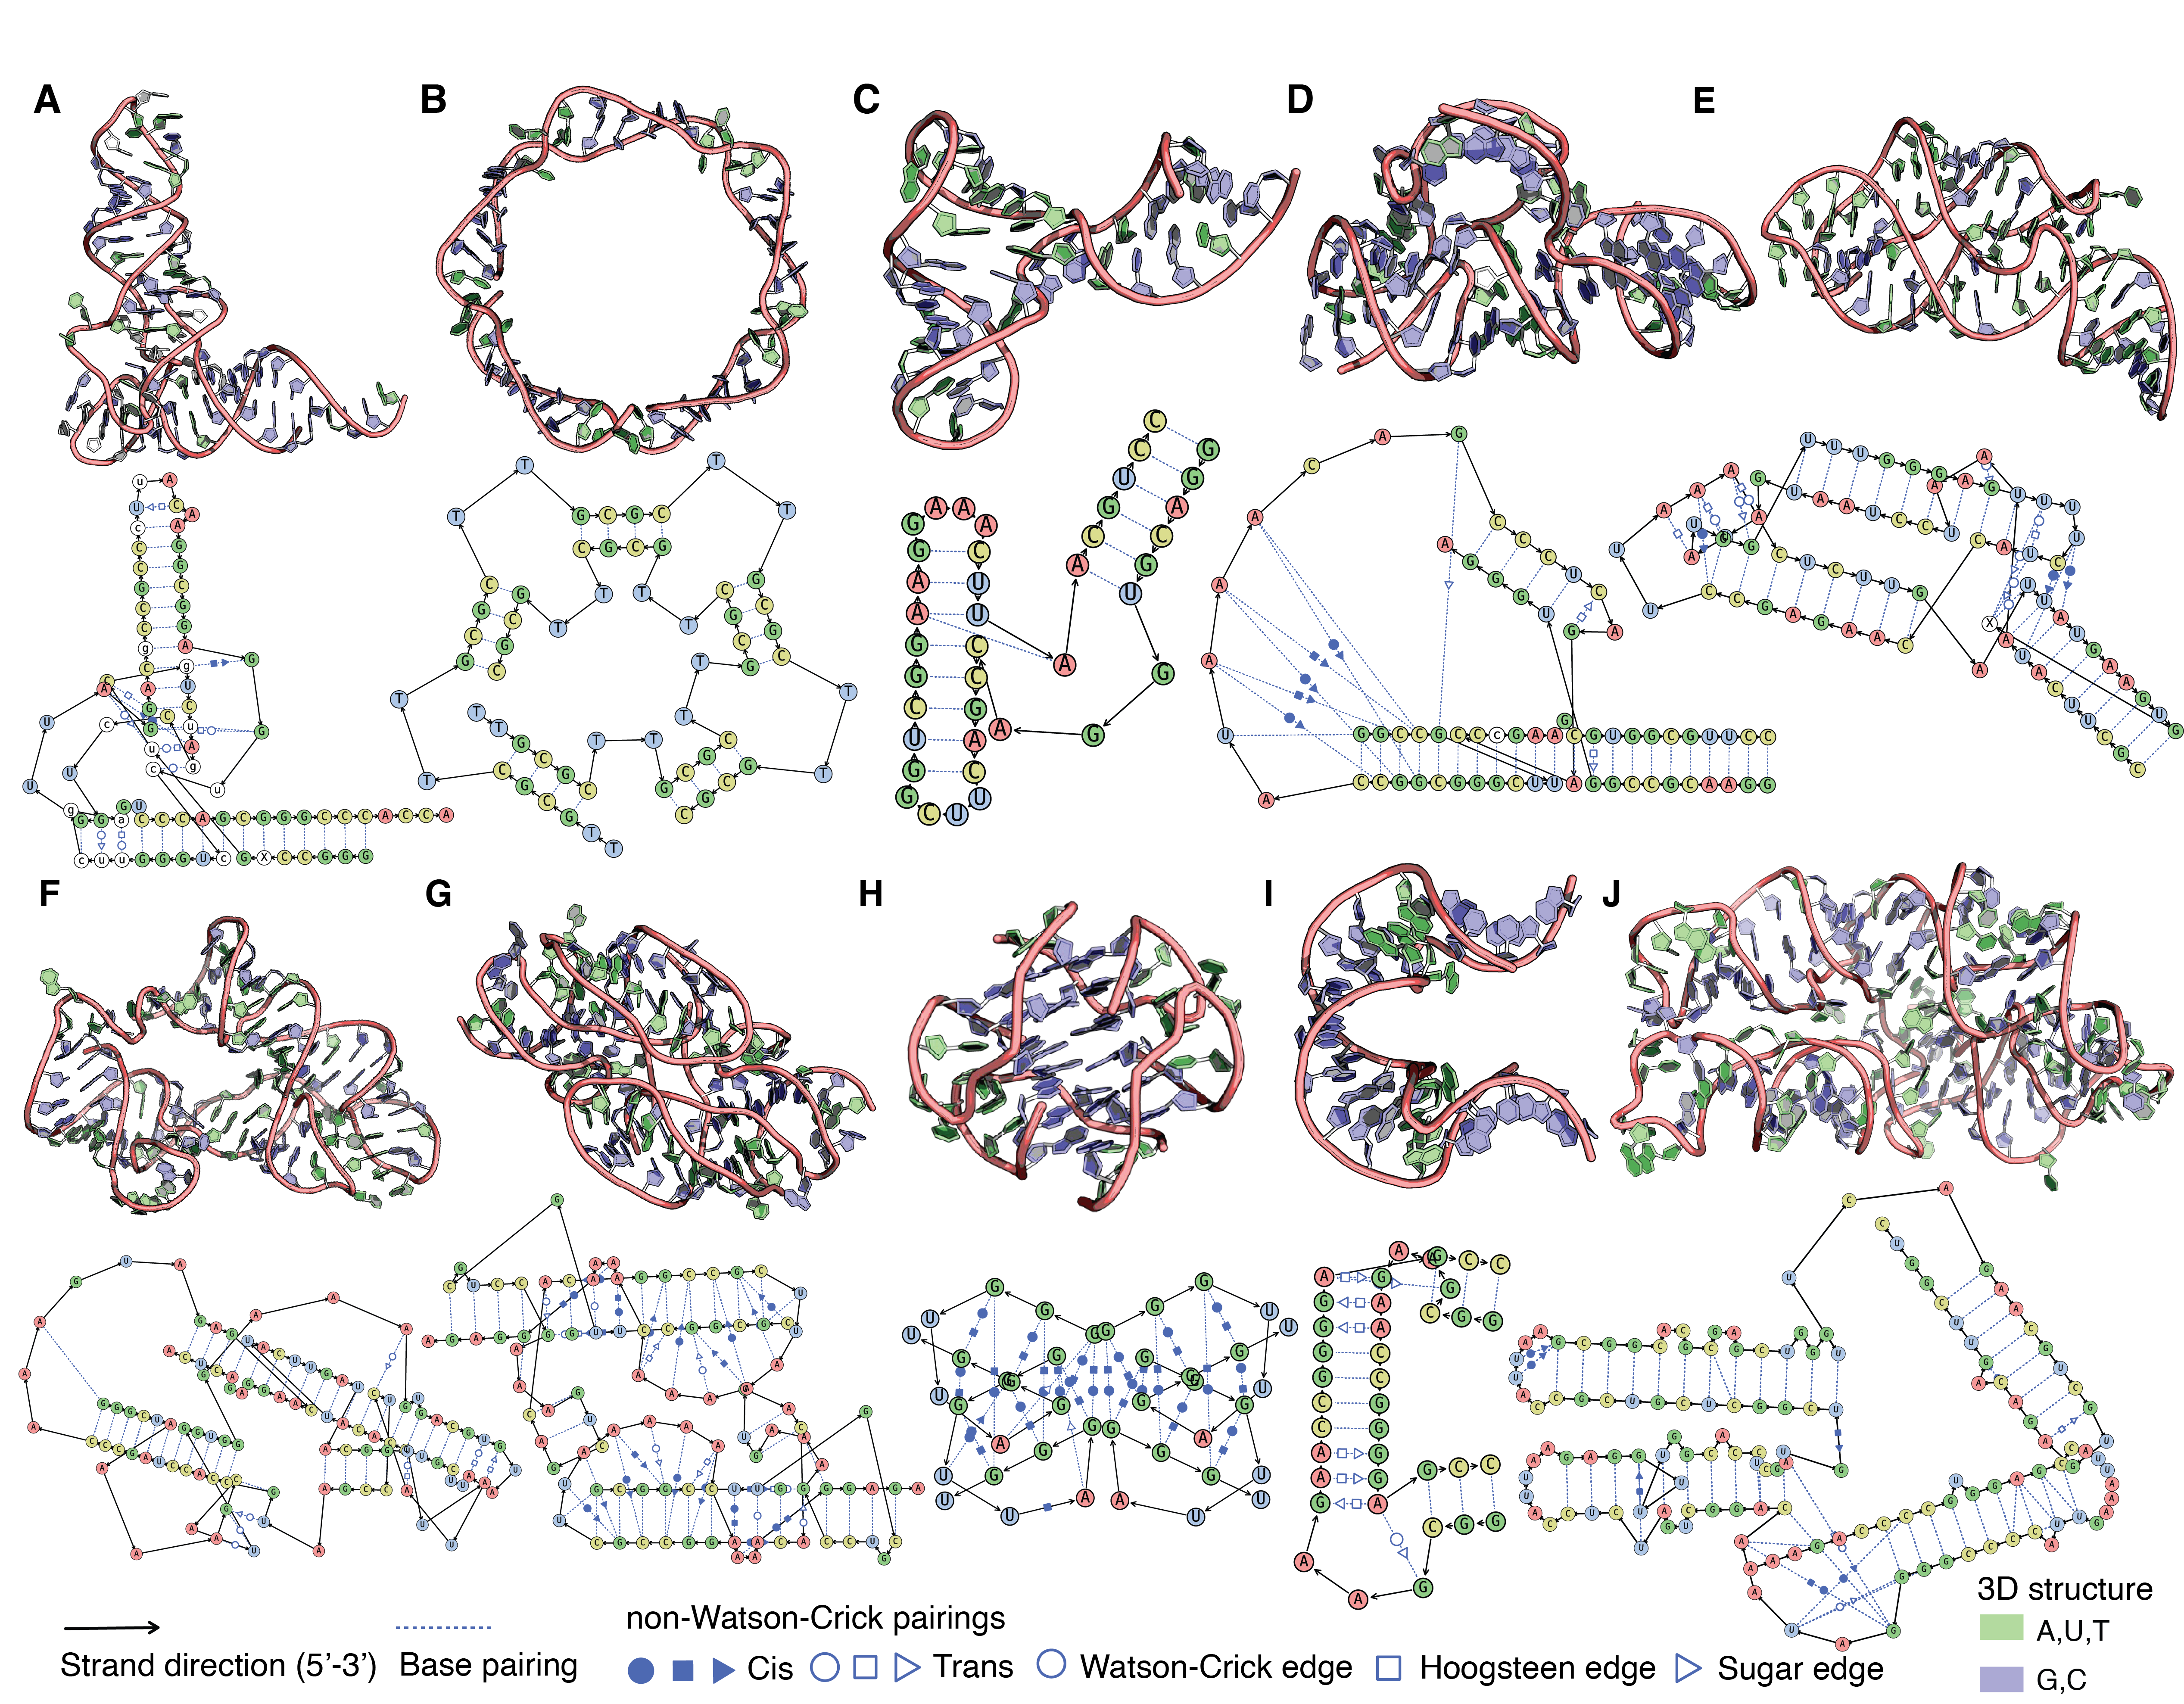
\includegraphics[width=0.8\paperwidth]{./rnascapefigs/figure1.png}}
 % archetecture.png: 1149x508 px, 72dpi, 40.53x17.92 cm, bb=0 0 1149 508
        \caption[RNAscape output for various structures from the PDB.]{\textbf{RNAscape output for various structures from the PDB.} The 3D structure at the top of each panel is from the PDB structure, with its corresponding RNAscape visualization shown below it. ({\bf A}) tRNA from Sulfolobus tokodaii (PDB ID: 7VNV), ({\bf B}) a single-stranded DNA molecule (PDB ID: 4NOE), ({\bf C}) Dengue virus RNA promoter (PDB ID: 7UMD), ({\bf D}) Pistol ribozyme (PDB ID: 6R47), ({\bf E}) Riboswitch from Escherichia coli (PDB ID: 1Y26), ({\bf F}) Cobalamin riboswitch regulatory element (PDB ID: 4FRN), ({\bf G}) NAD-II riboswitch (PDB ID: 8HBA), ({\bf H}) G-quadruplex (PDB ID: 2M18), ({\bf I}) RNA kink-turn motif (PDB ID: 7EFG) and ({\bf J}) the semi-symmetric peptidyl transferase center (PTC) of the large ribosomal subunit of Deinococcus radiodurans (PDB ID: 1NKW), also known as proto-ribosome (30). The molecular structure in (J) is shown along the two-fold pseudo-symmetry axis.}
  \label{fig:rnascape1}
\end{figure}
\end{center}
